\documentclass[varwidth=true, border=10pt, convert={size=640x}]{standalone}
\usepackage[utf8]{inputenc}
\usepackage{graphicx}
\usepackage{subcaption}
\begin{document}
\begin{figure}
 \centering
 \begin{subfigure}[b]{.32\textwidth}
 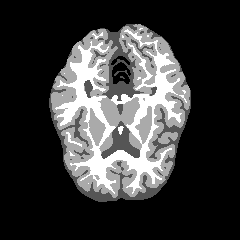
\includegraphics[width=.98\linewidth]{./images/lstmfeas_new_new.png}
 \subcaption{MD-LSTM}
 \end{subfigure}
  \begin{subfigure}[b]{.32\textwidth}
 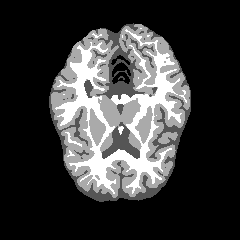
\includegraphics[width=.98\linewidth]{./images/grusfeas_new_new.png}
 \subcaption{MD-GRU}
  \end{subfigure}
  \begin{subfigure}[b]{.32\textwidth}
 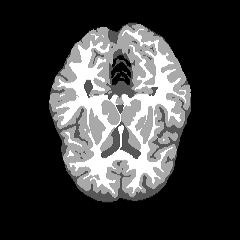
\includegraphics[width=.98\linewidth]{./images/Traindata5atslice19-Testlabel.png}
 \subcaption{Training labels}
  \end{subfigure}

  %\caption{Feasibility study. \emph{Top row:} slice 19 of the 5th training volume used for the evaluation. The images from left to right represent the results of the MD-LSTM, the MD-GRU and the manual labeling.}
\label{feasibilityqualitative}

\end{figure}

\end{document}
